\documentclass[jou]{apa6}

\usepackage[american]{babel}

\usepackage{csquotes}
\usepackage[style=apa,sortcites=true,sorting=nyt,backend=biber]{biblatex}
\DeclareLanguageMapping{american}{american-apa}
\addbibresource{bibliography.bib}


%%%%%%%%%%%%%%%%%%%%%%%%%%%%%%%%%%%%%%%%
%% Discrete Structures
%% The start of RBS stuff
%%%%%%%%%%%%%%%%%%%%%%%%%%%%%%%%%%%%%%%%

% Working internal and external links in PDF
\usepackage{hyperref}
% Extra math symbols in LaTeX
\usepackage{amsmath}
\usepackage{gensymb}
\usepackage{amssymb}
% Enumerations with (a), (b), etc.
\usepackage{enumerate}

\let\OLDitemize\itemize
\renewcommand\itemize{\OLDitemize\addtolength{\itemsep}{-6pt}}

\usepackage{etoolbox}
\makeatletter
\preto{\@verbatim}{\topsep=3pt \partopsep=3pt }
\makeatother

% These sizes redefine APA for A4 paper size
\oddsidemargin 0.0in
\evensidemargin 0.0in
\textwidth 6.27in
\headheight 1.0in
\topmargin -24pt
\headheight 12pt
\headsep 12pt
\textheight 9.19in



\setlength\parindent{0pt}

\title{Sample Quiz 4}
\author{Discrete Structures, Fall 2020}
\affiliation{RBS}

\leftheader{Discrete Sample Quiz 4}

\abstract{%
}

%\keywords{}

\begin{document}

\thispagestyle{empty}

\twocolumn
{\Large Preparation for Midterm - 1}

%Midterm might contain various types of tasks: 
%Computational Problems (applying algorithms in one
%particular situation); Analysis tasks (for example, 
%express something with predicates or quantifiers or apply some
%other conceptual knowledge); Proofs (showing that 
%some statement is always true). 

%Even, if you are following a known procedure or a proof pattern, 
%you need to add comments to explain what you are doing. 
%They can earn you some points, 
%even if your result turns out incomplete.

% Computation example (15 + 15 + 15 + 15)
% Analysis of a situation (20 + 20) 
% General proof (25 + 25)  

\section{Part A. Computational Problems}

In this part we apply known algorithms to particular situations. 
The goal is to obtain correct result and and add a short explanation, what 
you did and why.

\subsection{A1. Propositional Logic}

{\bf Question 1.} 
Consider this Boolean expression: $E = p \rightarrow q \rightarrow r$. 
Implication ($\rightarrow$) is right-associative. 
\begin{enumerate}[(a)]
\item Write an equivalent Boolean expression using only conjunctions ($\wedge$) and negations ($\neg$). 
\item Fill in the missing parts in the truth table:\\
\begin{tabular}{ c | c | c | c }
$p$ & $q$ & $r$ & $E$ \\ \hline
{\tt T} & {\tt T} & {\tt T} & $\ldots$ \\ \hline
{\tt T} & {\tt T} & {\tt F} & $\ldots$ \\ \hline
{\tt T} & {\tt F} & {\tt T} & $\ldots$ \\ \hline
{\tt T} & {\tt F} & {\tt F} & $\ldots$ \\ \hline
{\tt F} & {\tt T} & {\tt T} & {\tt T} \\ \hline
{\tt F} & {\tt T} & {\tt F} & {\tt T} \\ \hline
{\tt F} & {\tt F} & {\tt T} & {\tt T} \\ \hline
{\tt F} & {\tt F} & {\tt F} & {\tt T} \\ \hline
\end{tabular}
\end{enumerate}

\vspace{6pt}
{\bf Question 2.} 
Assume the following precedence order and associativity of the $5$ Boolean operations: 

\begin{tabular}{lll}
{\tt \textasciitilde{}a} & 1st precedence & right-associative \\
{\tt a/\textbackslash{}b} & 2nd precedence & right-associative \\
{\tt a\textbackslash{}/b} & 3rd precedence & right-associative \\
{\tt a<->b} & 4th precedence & left-associative \\
{\tt a->b} & 5th precedence & right-associative 
\end{tabular}

Show step-by-step how would you restore parentheses in the following 
Boolean expression (each step adds one pair of parentheses \textendash{}
in the order that follows from the rules of precedence 
and associativity):\\
{\tt a -> b /\textbackslash{} \textasciitilde{} c 
\textbackslash{}/ \textasciitilde{} \textasciitilde{} d 
<-> e -> f <-> g}





\subsection{A2. Sets and Quantifiers}

{\bf Question 3.} 
The universe $U$ is all integers between $1$ and $600$. 
$K_2 \subseteq U$ denotes all even numbers from $U$.
Similarly, $K_3 \subseteq U$ denotes all numbers divisible by $3$; 
$K_5 \subseteq U$ denotes all numbers divisible by $5$. 

\begin{enumerate}[(A)]
\item Draw Euler-Venn diagram with a big rectangle (the set $U$), 
the subsets $K_2$, $K_3$, $K_5$ as three intersecting circles.
\item Shade the region that corresponds to the set
$(K_2 \cap \overline K_3) \cup K_5$. 
\item Find the cardinality of the set
$\left| (K_2 \cap \overline K_3) \cup K_5 \right|$, 
justify your answer. 
\item Describe, which elements are in the set 
$(K_2 \cap \overline K_3) \cup K_5$ in English. 
For example: {\em ``All ... such that ... is divisible ... 
and/or is not divisible...''}. 
\end{enumerate}

\vspace{6pt}
{\bf Question 4.} 
In these pictures a red square on the intersection 
of row $i$ and column $j$ 
means that the predicate $L(i,j)$ is true (person $i$ 
loves person $j$). White square means that the predicate $L(i,j)$
is false. Here 
$i,j \in \{ \mathtt{a},\mathtt{b},\mathtt{c},\mathtt{d},\mathtt{e} \}$. 
\begin{center}
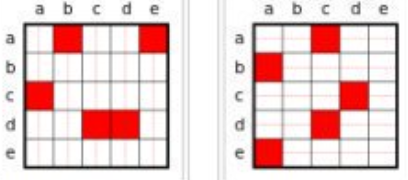
\includegraphics[width=2in]{midterm/predicate-grid.png}
\end{center}
Which statement is shown in the left picture?
\begin{enumerate}[(A)]
\item Everyone is loved by someone.
\item Eveyone loves someone.
\item Someone loves everyone.
\item Someone is loved by everyone.
\end{enumerate}
Which statement is shown in the right picture?
\begin{enumerate}[(A)]
\item $\forall x\, \exists y,\;L(y,x)$. 
\item $\forall x\, \exists y,\;L(x,y)$. 
\item $\exists x\, \forall y,\;L(x,y)$. 
\item $\exists x\, \forall y,\;L(y,x)$. 
\end{enumerate}






\subsection{A3. Algorithms and Big-O Notation}

In these problems you can verify the definition of the Big-O Notation 
or find the limit $f(n)/g(n)$ as $n \rightarrow \infty$. 

{\bf Question 5.} For each function find the smallest
$k$ such that $f(n)$ is in $O(n^k)$. Justify your answer.
\begin{enumerate}[(A)]
\item $f(n) = \sum_{j=1}^{n} (j^3 + j \log_2 j)$. 
\item $f(n) = n^3 + \sin n^7$. 
\item $f(n) = 1^2 + 2^2 + \ldots + n^2$.
\end{enumerate}

\vspace{6pt}
{\bf Question 6.} We say that the functions $f(n)$ and $g(n)$
{\em are of the same order}, if $f(n)$ is in $O(g(n))$ and
$g(n)$ is in $O(f(n))$. Find all pairs of functions in this 
list that are of the same order:
$$n^2 + \log_2 n,\; 2^n + 3^n,\; 100n^3 + n^2,\; n^2 + 2^n,$$
$$n^2 + n^3,\;3n^3 + 2^n.$$






\subsection{A4. Number Theory}


{\bf Question 7.}
\begin{enumerate}[(A)]
\item
Somebody has written a long hexadecimal number
{\tt F0F0F0...F0F} \textendash{} it uses $28$ digits "F"
separated by $27$ digits "0". 
Express the value of this number as a short expression
(without $\ldots$), using
the formula of a geometric progression: $\frac{b_1(q^{n+1}-1)}{q - 1}$. 
\item 
Somebody has written an infinite hexadecimal fraction 
{\tt 0.F0F0F0\ldots}. Express it as a rational number in 
decimal notation. 
\end{enumerate}



\vspace{6pt}
{\bf Question 8} 
\begin{center}
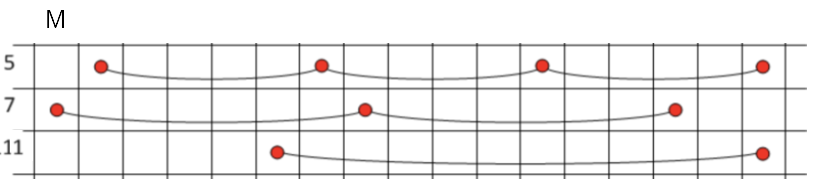
\includegraphics[width=3in]{midterm/sequences.png}
\end{center}

\begin{enumerate}[(A)]
\item Find some number $M \in \mathbb{Z}^{+}$ 
that gives the following remainders when divided by 
$5$, $7$ and $11$: 
$$\left\{
\begin{array}{l}
M \equiv 4\;(\text{mod}\,5)\\
M \equiv 0\;(\text{mod}\,7)\\
M \equiv 6\;(\text{mod}\,11)
\end{array} \right.$$
\item Find the arithmetic progression containing all such numbers $M$.
\end{enumerate}



\vspace{6pt}
{\bf Question 9.} 
\begin{enumerate}[(A)]
\item Alice has $13$-cent coins; Bob has $21$-cent coins. 
Alice wants to pay Bob exactly $1$ cent. How to do this?
\item Alice has $21$-cent coins; Bob has $13$-cent coins. 
Alice wants to pay Bob exactly $1$ cent. How to do this?
\item Solve the congruence equation \textendash{} find
$x$ such that $13x \equiv 1\;(mod\;21)$. 
\item Solve the congruence equation \textendash{} find
$x$ such that $13x \equiv 4\;(mod\;21)$. 
\end{enumerate}







\section{Part B. Analysis Tasks}

In these problems you have to apply concepts 
(such as predicates or quantifiers) to new situations, 
describe algorithms or procedures for new tasks
or sort cases in adaptive ways.


\subsection{B1. Propositional Logic}

{\bf Question 2.1.}
Among the people $A,B,C$ one is a truth-teller, 
the other two are liars. 
Every person ($A$, $B$, and $C$) has a closed box
in front of himself/herself. Exactly one of the 
boxes has a candy inside. $A,B,C$ know everything 
about each other and the location of candy.\\
Find out, which YES/NO questions you 
need to ask to find out, which box contains candy. 
Ask as few questions as possible 
(``brute-force'' strategies that ask clearly redundant
questions may only get partial credit). 

{\bf Question 2.2.} 
\begin{enumerate}[(a)]
\item Find out, if this formula is a tautology: 
$$\mathtt{((A \vee B) \wedge (A \rightarrow C) \wedge 
(B \rightarrow C)) \rightarrow C}.$$
\item Find out, if this formula is satisfiable: 
$$\mathtt{\neg (((A \vee B) \wedge (A \rightarrow C) \wedge 
(B \rightarrow C)) \rightarrow C)}.$$
\end{enumerate}

{\em Note.} A Boolean expression is called {\em tautology}, 
if it is true for all 
possible truth values of its variables. 
An expression is called {\em satisfiable}, 
if there is a way to assign 
variables so that it becomes true. 





\subsection{B2. Sets and Quantifiers}





%\vspace{6pt}
%{\bf Question 5.}
%Write the pseudocode of an algorithm that is finding ... 


%\vspace{6pt}
%{\bf Question 6.}



%\vspace{6pt}
%{\bf Question 7.}
%Is this mapping an injection? a surjection? a bijection? 
%(describe some combinatorial manipulation, where you match real-life situations with codes...)
%For example, you can match binary codes with words... polynomials... selections or permutations... 




%\vspace{6pt}
%{\bf Question 8.}
%Exercises with Scala precedence rules.
%Exercises with Scala left/right associativity. 
%Exercises with Scala short-circuit evaluation
%Exercises with Scala computing remainders etc. 
%Exercises with Scala notation of sets and set operations. 



%\vspace{6pt}
%{\bf Question 9.}
%Restore parentheses using precedence - you have Boolean operations of 5 %different levels of 
%complexity. 
%Restore syntax tree for the given Boolean expression... 



%\vspace{6pt}
%{\bf Question 10.}
%Logic puzzles with liars and truth-tellers. 


%\vspace{6pt}
%{\bf Question 11.}
%In a logic formula identify, which ones can be free, which are bound variables.
%Find, on which predicates this predicate expression acts. 
%What type of statement does it express, and explain your reasoning - why. 


%\vspace{6pt}
%{\bf Question 11.}
%In a sum notation, find how the sum can be expressed as an expression
%How would you calculate the 144th member of this sequence. How many %multiplication operations?






\section{Part C. Proofs}

In proof problems the goal is to prove some general statement by 
showing every essential step of your reasoning.
Below we describe various proof strategies and give some sample
statements that can be proven by that strategy.

{\bf Translate the problem into algebra}

In K.Rosen's textbook these are called ``direct proofs''
of IF-THEN statements. 
You assume that the condition is true, introduce some 

\begin{itemize}
\item If $n$ is odd, then $n^2$ is also odd. 
\item If the decimal notation of a number $n$ ends with the digit "5", 
then $n^2$ ends with digits "25". 
\end{itemize}

{\bf Reason by cases}

\begin{itemize}
\item $n^2 \equiv 5\;(\text{mod}\;11)$
if and only if\\
$n \equiv 4\;(\text{mod}\;11)$ 
or $n \equiv -4\;(\text{mod}\;11)$.
\item Assume that person $A$ says ``$B$ always lies.'' and 
person $B$ says ``We both always tell the truth.''.\\
It can happen only if $A$ tells the truth and $B$ lies
(you can analyze all other cases to see that only this works).
\end{itemize}


{\bf Proofs by Contradiction}

In these examples you assume that the statement is false
and get a contradiction.

\begin{itemize}
\item There are infinitely many primes.
\item There are infinitely many primes of the form $4n+3$. 
\item Assume that there are infinitely many primes
that divide some value of the polynomial 
$P(n) = n^2 + n + 1$. 
\item $\sqrt{2}$ is irrational.
\item $\log_2 10$ is irrational.
\end{itemize}

{\bf Building Bijective Functions}

Any combinations of these tactics can be used
to prove that two sets have the same cardinality
(and that there is a bijective function from one set to another).

\begin{itemize}
\item There is a bijection from $\mathbb{Z}^{+} \cup \{ 1,2,\ldots,n \}$
to $\mathbb{Z}^{+}$ (one can add $n$ new guests to the Hilbert's hotel). 
\item There is a bijection from $\mathbb{Z}^{+} \times \{ 1,2 \}$
to $\mathbb{Z}^{+}$ (if there are two infinite buses with guests: 
$(1,1),(2,1),(3,1),\ldots$ and $(1,2),(2,2),(2,3),\ldots$, 
then they can be hosted in a single Hilbert's hotel). 
\item There is a bijection from $\mathbb{Z}^{+} \times \mathbb{Z}^{+}$
to $\mathbb{Z}^{+}$ (infinitely many infinite buses can be hosted in a 
single Hilbert's hotel). 
\item There is a bijection from $\mathbb{Q}$ to $\mathbb{Z}^{+}$. 
\end{itemize}

For subsets of real numbers you might need different 
proof methods: 

\begin{itemize}
\item There is a bijective function from any closed 
segment $[a;b]$ to any other closed segment $[c;d]$ 
(regardless of their lengths). Can be achieved by a linear
function. 
\item There is a bijective function from any open 
segment $(a;b)$ to any other open segment $(c;d)$. 
\item There is a bijective function from any open 
segment $(a;b)$ to the set of all real numbers $\mathbb{R}$
or to the half-line of all positive reals $(0;+\infty)$. 
\item There is a bijective function from a 
semi-open segment $[0;1)$ to an open segment $(0;1)$. 
\end{itemize}


{\bf Proving that there is no Bijection}

\begin{itemize}
\item Numbers on $(0;1)$ are uncountable. (Cantor's diagonalization). 
\item All real numbers $\mathbb{R}$ are uncountable - there 
is no bijection from $\mathbb{R}$ to $\mathbb{Z}^{+}$ or
to $\mathbb{Q}$. 
\item All infinite sequences of integers are uncountable
(Proof by Cantor's diagonalization). 
\item All non-decreasing sequences of integers are uncountable. 
\item The Power-set of any countable set is 
uncountable. For example, 
there is no bijection from $\mathcal{P}(\mathbb{Z}^{+})$
to $\mathbb{Z}^{+}$ (i.e. no mapping from the set of all subsets of 
positive integers to the set of integers themselves).
\end{itemize}




\end{document}

